\section{Acceso al sistema}

  \paragraph{}Para acceder al sistema, lo primero que debemos hacer es abrir
  un navegador de internet e introducir la dirección URL que apunta a la
  pantalla inicial de nuestra aplicación. Si ha seguido los pasos de instalación
  de la aplicación del capítulo \ref{instalacion},
  \textit{Proceso de Instalación}, esta URL será
  \textit{http://localhost/asesorias}, y debe mostrarse tal y como aparece en la
  figura \ref{capturaPaginaInicial}.

  \paragraph{}En primer lugar, introduzca el nombre de usuario con el cual desea
  acceder al sistema en la caja de texto que ilustra la figura
  \ref{capturaCajaTextoNombre}.

  \begin{figure}[!ht]
    \begin{center}
      \fbox{
      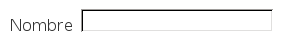
\includegraphics[]{4.Funcionamiento_Aplicacion/4.2.Acceso_Sistema/Capturas/caja_texto_nombre.png}
      }
      \caption{Captura de pantalla de la caja de texto para introducir el nombre.}
      \label{capturaCajaTextoNombre}
    \end{center}
  \end{figure}

  \paragraph{}Seguidamente, introduzca la contraseña para el usuario introducido
  en el paso anterior en la caja de texto que ilustra la figura
  \ref{capturaCajaTextoPassword}.

  \begin{figure}[!ht]
    \begin{center}
      \fbox{
      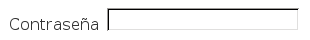
\includegraphics[]{4.Funcionamiento_Aplicacion/4.2.Acceso_Sistema/Capturas/caja_texto_password.png}
      }
      \caption{Captura de pantalla de la caja de texto para introducir la contraseña.}
      \label{capturaCajaTextoPassword}
    \end{center}
  \end{figure}

  \paragraph{}Para poder acceder al sistema con el nombre de usuario y
  contraseña proporcionadas, hay que elegir con que rol se desea participar en
  el sistema. Hay un rol por cada tipo de usuario que participa en el sistema;
  es decir, \textit{Administrador principal}, \textit{Administrador de centro},
  \textit{Asesor} y \textit{Alumno}. La elección del rol condicionará la zona de
  la aplicación a la que se accederá.

  \paragraph{}Para seleccionar el rol con el que se desea acceder al sistema,
  habrá que elegirlo entre las opciones que ofrece la lista desplegable, tal y
  como lo ilustra la figura \ref{capturaListaDesplegableRol}.

  \begin{figure}[!ht]
    \begin{center}
      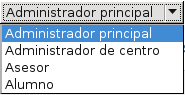
\includegraphics[]{4.Funcionamiento_Aplicacion/4.2.Acceso_Sistema/Capturas/lista_desplegable_rol.png}
      \caption{Captura de pantalla de la lista desplegable para elegir rol.}
      \label{capturaListaDesplegableRol}
    \end{center}
  \end{figure}

  \paragraph{}Una vez elegido el rol con el que se desea acceder, se pulsará
  el botón \textit{OK} que muestra la figura \ref{capturaBotonOK}, o se pulsará
  la tecla \textit{Intro} del teclado para intentar realizar el acceso.

  \begin{figure}[!ht]
    \begin{center}
      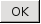
\includegraphics[]{4.Funcionamiento_Aplicacion/4.2.Acceso_Sistema/Capturas/boton_ok.png}
      \caption{Captura de pantalla del botón OK.}
      \label{capturaBotonOK}
    \end{center}
  \end{figure}

  \paragraph{}Nótese que para que el acceso al sistema sea efectivo, debe
  existir con anterioridad, en la base de datos de la aplicación, tanto el
  usuario como la contraseña introducidas, con permiso para el tipo de rol con
  el que se intenta acceder.

  \subsection{Recordar contraseña}

  \paragraph{}En el caso de que dispongamos de un usuario válido para acceder a
  la aplicación pero hemos olvidado la contraseña, es posible generar una nueva,
  que será enviada al correo electrónico del usuario.

  \paragraph{}Para ello, en la pantalla inicial debemos pulsar el enlace
  \textit{Recordar contraseña}, que se encuentra a la derecha del botón
  \textit{OK} \ref{capturaBotonOK}. La imagen \ref{capturaRecordarPassword}
  muestra el enlace mencionado.

  \begin{figure}[!ht]
    \begin{center}
      \fbox{
      
\includegraphics[]{4.Funcionamiento_Aplicacion/4.2.Acceso_Sistema/4.2.1.Recordar_Password/Capturas/recordar_password.png}
      }
      \caption{Captura de pantalla del enlace \textit{Recordar contraseña}.}
      \label{capturaRecordarPassword}
    \end{center}
  \end{figure}

  \paragraph{}Una vez pulsado, la aplicación pedirá el correo electrónico del
  usuario para el cual se desea recuperar la contraseña de acceso, como se puede
  ver en la imagen \ref{capturaPedirCorreo}.

  \begin{figure}[!ht]
    \begin{center}
      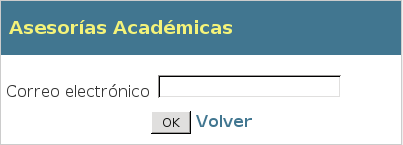
\includegraphics[]{4.Funcionamiento_Aplicacion/4.2.Acceso_Sistema/4.2.1.Recordar_Password/Capturas/pedir_correo.png}
      \caption{Captura de pantalla de la petición del correo electrónico para recuperar la contraseña.}
      \label{capturaPedirCorreo}
    \end{center}
  \end{figure}

  \paragraph{}Si introducimos un correo electrónico válido, que esté asociado a
  un usuario de la base de datos de la aplicación, y pulsamos el botón
  \textit{OK} \ref{capturaBotonOK}, aparecerá un mensaje diciendo que la nueva
  contraseña se ha generado con éxito, la cual habrá sido enviada al correo
  electrónico introducido. Se puede ver una captura de pantalla de este mensaje
  en la imagen \ref{capturaPedirCorreoExito}.

  \begin{figure}[!ht]
    \begin{center}
      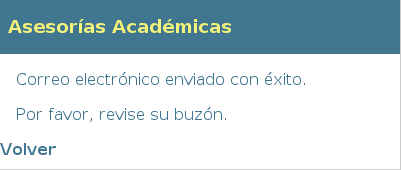
\includegraphics[]{4.Funcionamiento_Aplicacion/4.2.Acceso_Sistema/4.2.1.Recordar_Password/Capturas/pedir_correo_exito.png}
      \caption{Captura de pantalla del mensaje con éxito al recuperar la contraseña.}
      \label{capturaPedirCorreoExito}
    \end{center}
  \end{figure}